\documentclass[final,5p,times,twocolumn]{elsarticle}

\usepackage{amsmath}
\usepackage{amssymb}
\usepackage{graphicx}
\usepackage{hyperref}
\usepackage{multirow}

\journal{Smart Agricultural Technology}

\begin{document}

\begin{frontmatter}

\title{Automated Phenotypic Trait Extraction from Longitudinally Sectioned Chili Pepper Fruits Using Instance Segmentation}
%%Anh Tuấn kêu điền dô nma chưa nghĩa ga :>
%% BỎ TRỐNG TOÀN BỘ PHẦN \author Ở ĐÂY (DOUBLE ANONYMIZED PEER REVIEW)

%% Tác giả 1
\author[1,2]{Thuy Nguyen Thi Nhu\fnref{fn1}}
\ead{24521755@uit.edu.vn}

%% Tác giả 2
\author[1,2]{Trong Tai Ha\fnref{fn1}}
\ead{21520436@uit.edu.vn}

\author[1,2]{Chau Anh Le\fnref{fn1}}
\ead{21511821@uit.edu.vn}

%% Tác giả 3
\author[1,2,3]{Thanh Tuan Thai}
\ead{tuantt@uit.edu.vn}

%% Tác giả 4
\author[1,2]{Tien Dung Mai}
\ead{dungmt@uit.edu.vn}

%% Tác giả 6 (Corresponding)
\author[3]{Yong Suk Chung\corref{cor1}}
\ead{yschung@jejunu.ac.kr}

%%%%%% Affiliations %%%%%%
\address[1]{Faculty of Computer Science, University of Information Technology, Ho Chi Minh city 70000, Vietnam}
\address[2]{Vietnam National University, Ho Chi Minh city 70000, Vietnam}
\address[3]{Department of Plant Resources and Environment, Jeju National University, Jeju 63243, Republic of Korea}

%%%%%% Chú thích & Tác giả liên hệ %%%%%%
\cortext[cor1]{Address correspondence to: yschung@jejunu.ac.kr (Y.S.C.); thanhnd@uit.edu.vn(N.D.T)}
\fntext[fn1]{These authors contributed equally to this work.}
\begin{abstract}
In recent years, the intersection of computer vision and precision agriculture has led to significant advancements. Accurate measurement of chili pepper phenotypes, particularly complex internal structures, plays a pivotal role in modern agricultural genetics and cultivar development. However, traditional manual measurements and most existing computer vision approaches primarily focus on external fruit morphology, resulting in a critical lack of comprehensive data on internal cross-sections. To address this limitation, this study proposes an automated framework to extract phenotypic metrics from vertically cross-sectioned chili pepper images. The proposed pipeline isolates individual fruits from a standardized black background using a YOLOv7 detector, with threshold-based localization retained as a configurable fallback. Subsequently, a YOLOv8m instance segmentation model is employed to delineate five key classes: whole fruit, outer, endocarp, a composite placenta--pedicel region, and seed. Experimental evaluations demonstrate the model's strong performance, achieving a Precision of 93.10\%, a Recall of 91.90\%, and a mask mean Average Precision (mAP@0.5) of 94.20\% in segmenting these complex and heavily occluded internal features. Leveraging these high-quality masks, the system automatically computes a comprehensive set of internal phenotypic parameters. Ultimately, this research presents a robust morphological analysis framework that overcomes the limitations of manual methods, establishing a reliable quantitative database for precision agriculture applications.
\end{abstract}


\begin{keyword}
Chili pepper \sep Instance segmentation \sep YOLOv8m \sep Phenotyping \sep Computer vision \sep Smart agriculture
\end{keyword}

\end{frontmatter}

\section{Introduction}

Precision agriculture and data-driven crop breeding have attracted increasing attention, with computer vision and machine learning becoming important tools for high-throughput plant phenotyping \cite{CV, ML}. A major challenge in this field is the accurate and efficient quantification of complex phenotypic traits at a fine-grained level. Such quantitative phenotypic information can help characterize genetic variation and support the selection and development of improved crop cultivars.

For chili peppers (\textit{Capsicum} spp.), an economically important crop with substantial phenotypic and genetic diversity, fruit traits are important targets for characterization and breeding \cite{tripodi}. Internal fruit tissues are particularly relevant to commercially and biologically important characteristics. For instance, the placenta is generally considered the main site of capsaicinoid biosynthesis, although capsaicinoid-related activity may also be detected in other fruit tissues depending on genotype and developmental stage. Furthermore, mesocarp thickness is another important fruit morphology trait directly related to fruit firmness, processing quality, and yield.

Several existing computer vision studies on chili peppers primarily extract external traits, including overall fruit size, shape, and color. While these external metrics are valuable, the automated quantification of internal longitudinal cross-sectional structures remains comparatively underexplored. Traditional manual measurements of these internal regions are labor-intensive, destructive, and prone to human error, highlighting a critical need for automated solutions.

Extracting features from longitudinal cross-sections presents unique technical challenges. In particular, seed clusters are densely distributed and frequently overlap, creating substantial occlusion that complicates accurate counting and area estimation. Consequently, pixel-level instance segmentation is more appropriate than simple object detection when the objective is to precisely quantify the geometry, boundary, and area of individual anatomical structures within the fruit.

To address these challenges, our study introduces a fully automated framework for extracting comprehensive phenotypic parameters from longitudinal cross-sectional images of chili peppers. The framework integrates a preliminary preprocessing stage for individual fruit localization and orientation normalization with a YOLOv8m-based instance segmentation model as the core analytical component. Although the neural network is trained to identify five distinct classes, the runtime pipeline deliberately employs a straightforward thresholding approach to isolate the whole chili body. This design choice avoids unnecessary computational complexity, demonstrating that traditional techniques remain highly effective for segmenting easily distinguishable boundaries. Consequently, the YOLOv8m model is dedicated exclusively to the accurate segmentation of the intricate internal components: the endocarp, the composite placental region, the seeds, and the outer region (a non-planar artifact resulting from the three-dimensional fruit structure visible in cross-section). By synthesizing these segmentation masks with deterministic geometric algorithms, the proposed framework provides a robust quantitative basis for the morphological analysis of longitudinally cross-sectioned chili pepper fruits, contributing to more efficient phenotypic characterization in modern breeding programs.



\section{Materials and Methods}

The overall workflow of the proposed automated chili phenotyping framework is illustrated in Fig.~\ref{fig:overall_pipeline}. The system operates through a sequential pipeline comprising four primary stages: image acquisition and dataset preparation, automated bounding box cropping, instance segmentation of internal anatomical structures, and the automated extraction of quantitative phenotypic traits. The detailed methodologies for each of these stages are elaborated in the subsequent subsections.

\begin{figure*}[htbp]
\centering
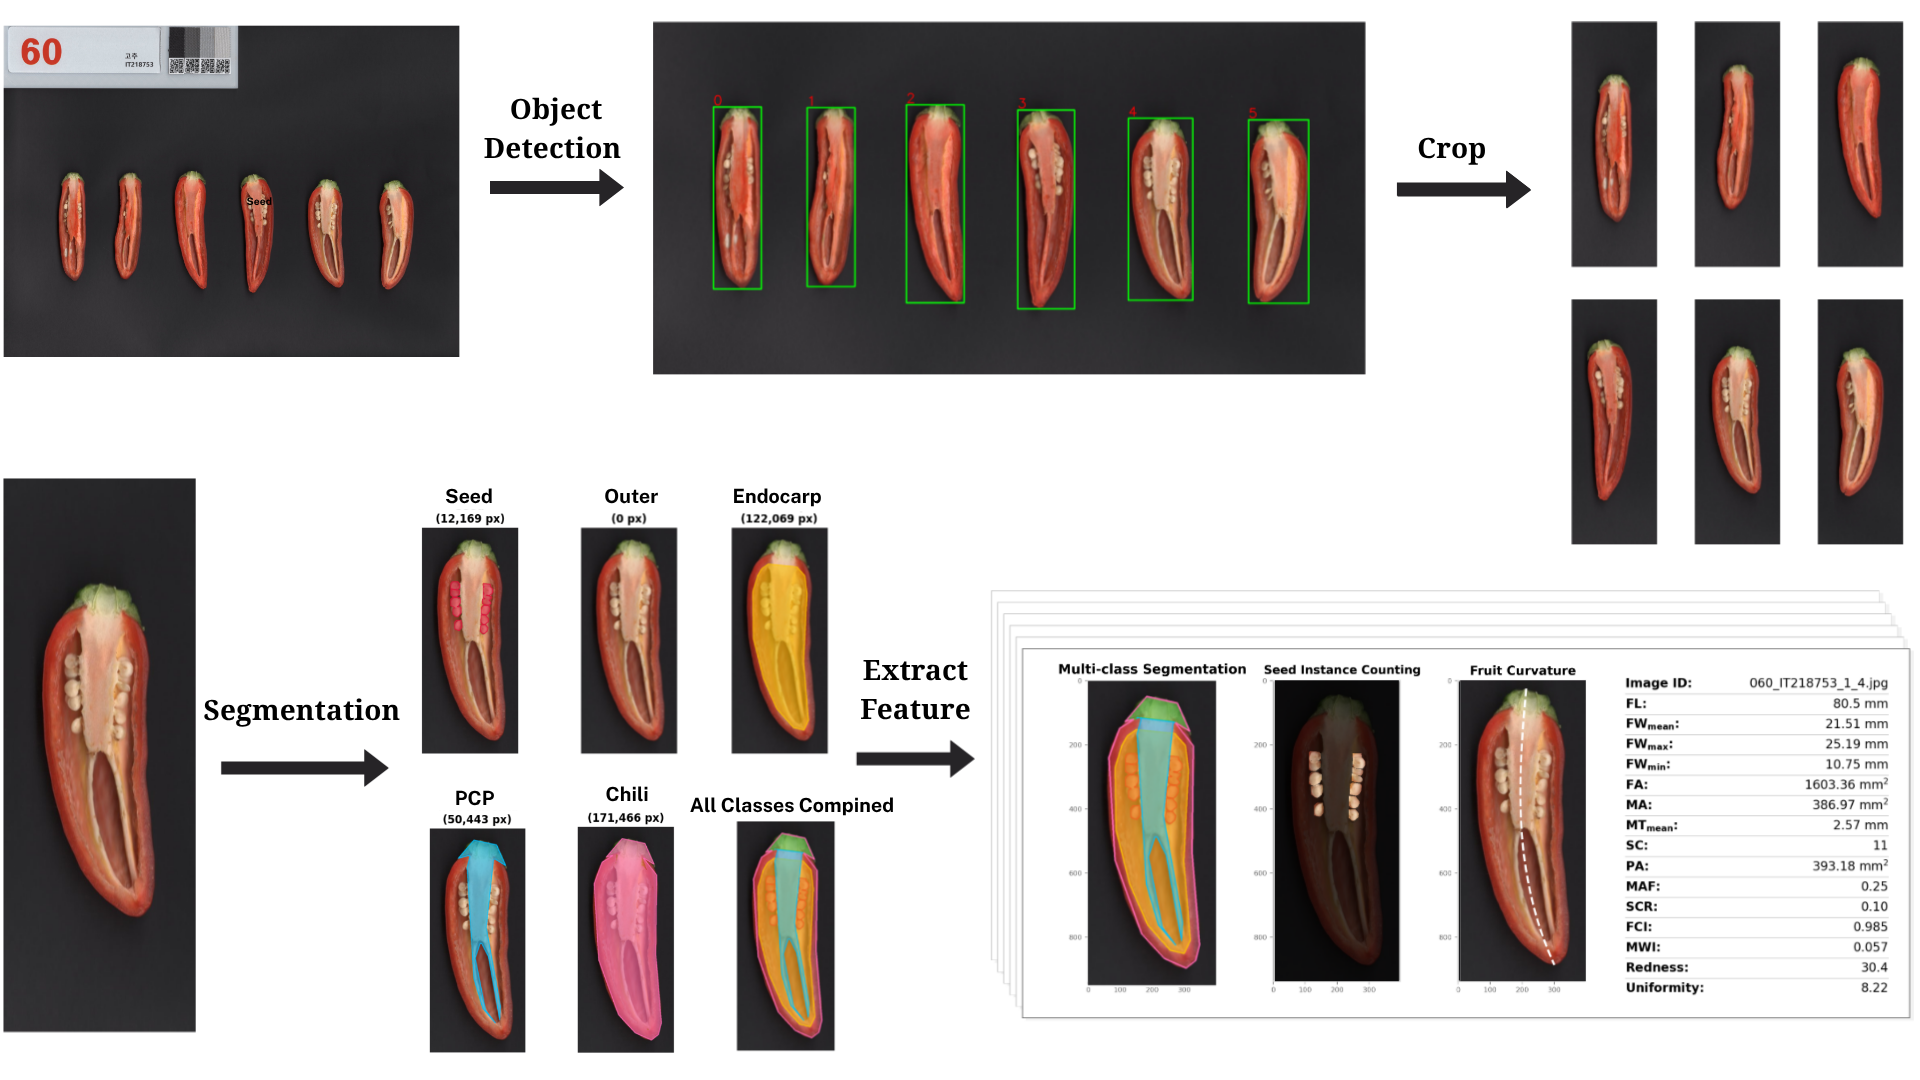
\includegraphics[width=\textwidth]{images/Pipeline_final.png}
\caption{Overall Pipeline}
\label{fig:overall_pipeline}
\end{figure*}



\subsection*{Dataset and plant materials}
The dataset used in this study comprises 386 chili pepper (\textit{Capsicum annuum}) accessions obtained from the Korean Gene Bank, consisting of two accession sets: 56 advanced breeding lines and 330 consumer-type (landrace)
cultivars, representing diverse geographical origins and a broad range of genetic and morphological variation. To ensure that differences in internal fruit anatomical structure were genotype-driven rather than environmentally induced, all accessions were cultivated simultaneously under identical,
controlled greenhouse conditions, following a randomized block design: each
accession was grown as a plot of six plants, with plot position randomized
across the field, and each plot replicated three times across three separate
greenhouses (18 plants per accession in total), minimizing systematic error.



During cultivation and sample collection, some plants died, some accessions on the initial list were not planted, and diseased plants were excluded from sampling. Consequently, usable fruit images were not obtained from all 386 initial accessions. The final dataset comprised 367 original multi-fruit images from 285 accessions. The data were partitioned into training, validation, and test sets at the accession level, ensuring that all images from a given accession belonged to only one set. These sets contained 262, 47, and 58 original images, respectively; after individual-fruit cropping, the corresponding numbers of fruit images were 1237, 264, and 264.


\subsection*{Image acquisition and spatial calibration}

Longitudinal fruit sections were photographed under standardized lighting, camera-to-sample distance, and viewing angle to maintain consistency across images. Each image included a white-balance reference patch and a QR code of known dimensions ($10 \times 10$\,mm), used as a calibration reference to convert measurements from pixels to millimetres. When the QR code is detected and decoded, the system determines the conversion factor from its dimensions in the image and its corresponding physical dimensions. If QR decoding fails, the system uses the dataset-level mean scale as a fallback and records the source of the applied scale. The use of a reference object of known dimensions to convert image measurements into physical units is consistent with established methods in plant image analysis \cite{cass}.

Letting $(w_{QR}, h_{QR})$ denote the pixel width and height of the decoded QR code's bounding box, the calibration factor $\gamma$ (mm/pixel) is computed as:
\begin{equation}
    \gamma = \frac{10}{(w_{QR} + h_{QR})/2} \quad (\text{mm/pixel})
\end{equation}

Using $\gamma$, length and area measurements are converted to their corresponding physical units as follows:
\begin{equation}
 L_{\mathrm{mm}} = L_{\mathrm{px}} \gamma,\qquad
 A_{\mathrm{mm}^2} = A_{\mathrm{px}} \gamma^{2}.
\end{equation}




\noindent Here, $L_{\mathrm{px}}$ is the length in pixels and $A_{\mathrm{px}}$ is the area in pixels$^2$.


\subsection*{Training Data Preparation and Annotation Protocol}
To prepare the segmentation dataset, original images containing multiple fruits were processed to isolate individual longitudinal fruit sections. Fruit localization used a YOLOv7-based object detection model \cite{yolov7}, adopted from a previous study \cite{ver1}. The predicted bounding boxes were expanded with a surrounding margin before cropping to reduce the risk of excluding fruit parts extending beyond the boxes.

The individual-fruit images were then imported into Label Studio for manual polygon annotation of four target classes:
\begin{itemize}
    \item \textbf{Outer}: The part of the fruit outside the cut plane that remains visible in the image due to the three-dimensional structure of the fruit.
    \item \textbf{Endocarp}: The entire region enclosed by the endocarp boundary in the fruit section, including locations occupied by the placenta and seeds.
    \item \textbf{PCP (placenta--pedicel composite)}: The composite region comprising the placenta and its attached pedicel.
    \item \textbf{Seed}: Seeds were annotated as separate instances according to their visible portions in the image. For overlapping seeds, only the observable portion of each seed was annotated, without inferring occluded regions.
\end{itemize}

For indistinct boundary segments, annotators estimated the boundary position using changes in color, texture, and continuity with neighboring boundary segments. All annotations were reviewed by at least two people to assess consistency and identify annotation errors.



\begin{figure}[htbp]
    \centering
    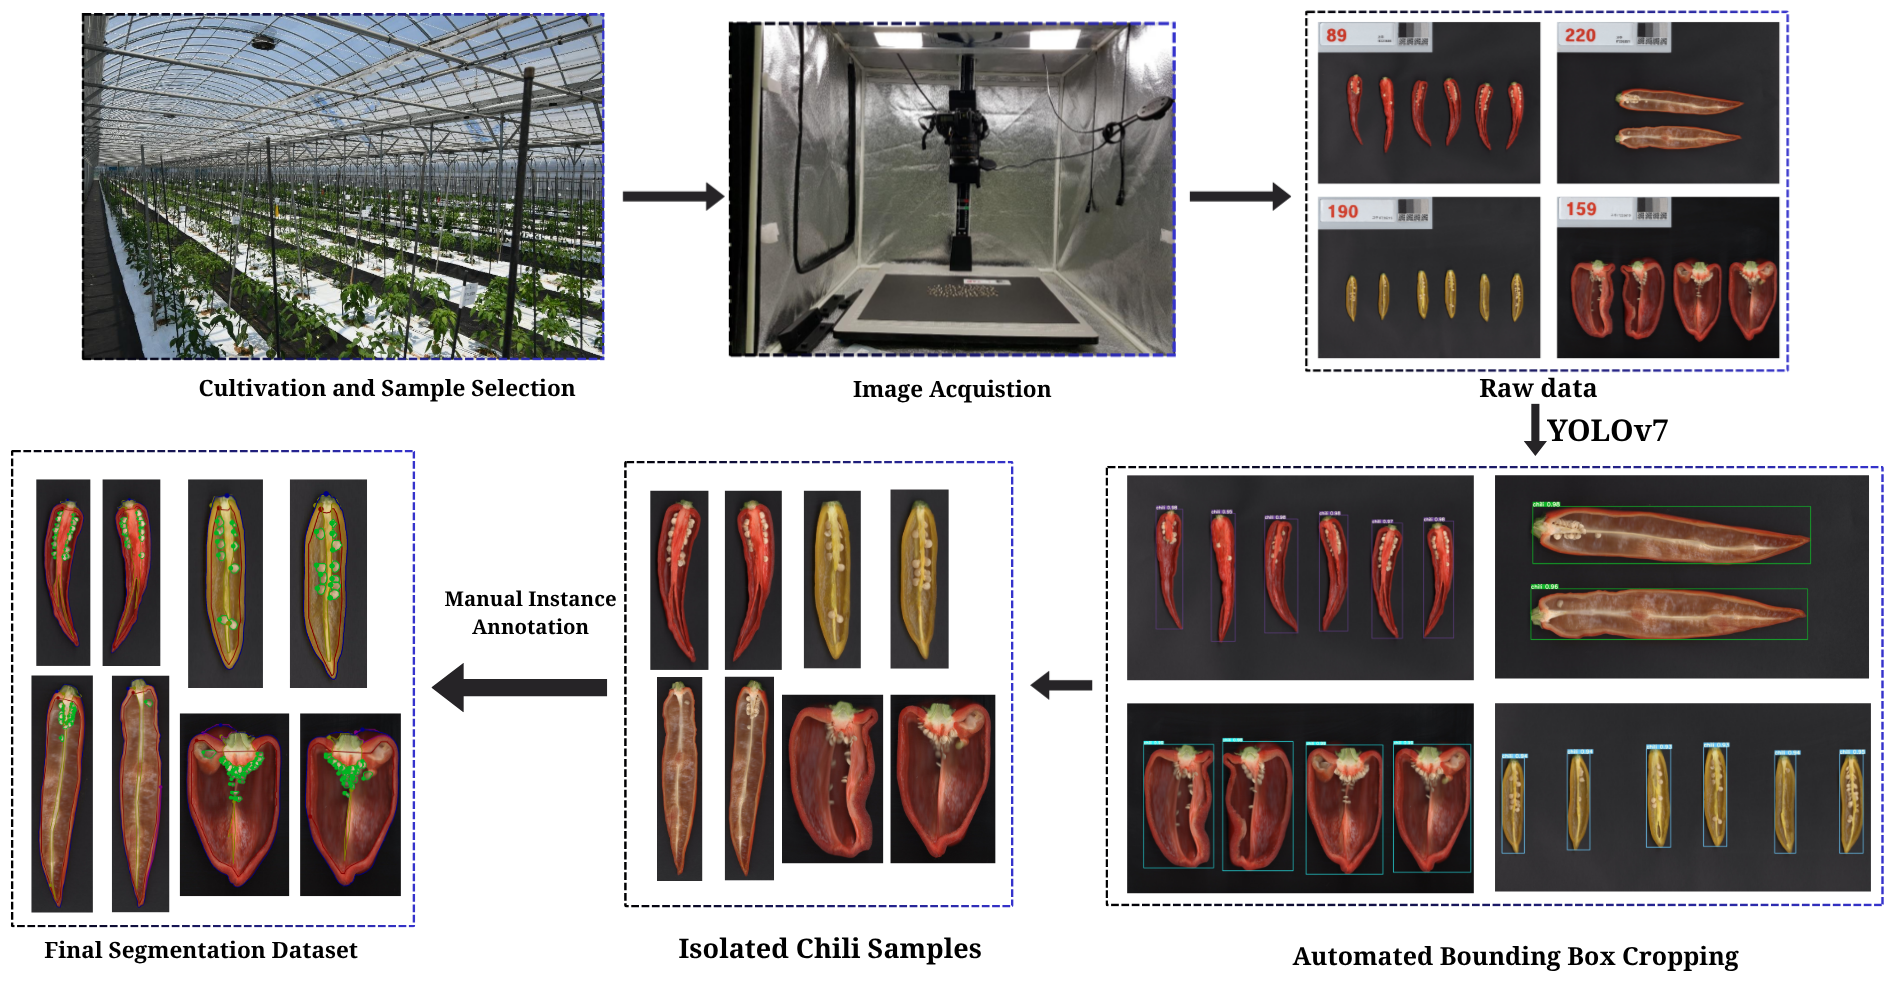
\includegraphics[width=\linewidth]{images/Chili.png}
    \caption{\textbf{Image acquisition and dataset construction workflow for longitudinal chili fruit section segmentation.} The plants were grown in greenhouses, and fruit sections were photographed using a camera system under standardized conditions. From original images containing multiple fruits, YOLOv7 localizes individual fruits with bounding boxes; these boxes are expanded with a surrounding margin before cropping into individual-fruit images. The resulting images are manually annotated using polygons for four classes: outer, endocarp, PCP (placenta--pedicel composite), and seed.}
    \label{fig:preprocessing_workflow}
\end{figure}


\subsection*{Instance segmentation model and training configuration}
This study uses YOLOv8m-seg [REF] to segment four target classes in individual chili fruit images. The model is initialized with weights pretrained on the COCO dataset [REF] and fine-tuned on the annotated dataset of this study. The training, validation, and test sets follow the accession-level partitioning described in the dataset section. During training, data augmentations include horizontal flipping, vertical flipping, rotation within $\pm15^{\circ}$, and Mosaic. All models in the architecture comparison in Section 3.1 are trained and evaluated using the same input size, configured as \texttt{imgsz=960}.

\subsection*{Inference and Mask Generation for Trait Extraction}

The inference pipeline converts an input image containing multiple fruits into individual-fruit images and their corresponding structural masks, providing the basis for phenotypic trait extraction. The system combines fruit localization using YOLOv7, instance segmentation using YOLOv8m-seg, and a thresholding method adopted from the previous study to generate the whole-fruit mask. Together, these outputs describe the fruit extent and anatomical components, supporting the construction of measurement regions appropriate for each trait.

First, YOLOv7 localizes individual fruits in the input image. For the standardized image layout used in this study, the header region containing labels and the calibration marker is excluded from the fruit search region. The remaining image region is resized while preserving its aspect ratio and padded to match the model input. Predicted bounding boxes are filtered by confidence and overlap to remove duplicate detections. The retained boxes are expanded with a surrounding margin before cropping to reduce the risk of excluding fruit parts extending beyond the boxes.

Each individual-fruit image is then processed by YOLOv8m-seg to segment four target classes: outer, endocarp, PCP, and seed. Predictions are filtered by confidence and overlap and then converted into the corresponding binary masks: $M_{\mathrm{outer}}$ represents the fruit region outside the cut plane; $M_{\mathrm{endocarp}}$ represents the region segmented by the model as endocarp; $M_{\mathrm{PCP}}$ represents the composite placenta--pedicel region; and $M_{\mathrm{seed}}$ represents the union of the retained seed regions. Individual seed instance masks are also stored separately for subsequent seed-count estimation.

The initial segmentation also supports orientation normalization of elongated, horizontally positioned fruits. For an image whose width exceeds 1.5 times its height and for which a PCP prediction is available, the centroid of the largest PCP instance determines the rotation direction: the image is rotated by $90^{\circ}$ clockwise if the centroid lies in the left half, or counterclockwise if it lies in the right half. Segmentation is repeated on the rotated image to obtain masks corresponding to the new orientation. Images that do not meet these conditions retain their original orientation; the pipeline does not apply a $180^{\circ}$ rotation.

Following orientation normalization, the whole-fruit mask $M_{\mathrm{chili}}$ is generated independently using the red-channel thresholding method adopted from the previous study \cite{ver1}. The thresholded mask undergoes morphological closing, after which the largest external contour is retained and filled to obtain $M_{\mathrm{chili}}$. This mask represents the whole-fruit extent and may include both the outer region and the pedicel.

The masks $M_{\mathrm{outer}}$, $M_{\mathrm{endocarp}}$, $M_{\mathrm{PCP}}$, and $M_{\mathrm{seed}}$ are clipped to $M_{\mathrm{chili}}$ before subsequent processing. The mask $M_{\mathrm{PCP}}$ is processed to separate the pedicel from the placenta using the method described in the next subsection. The whole-fruit and component masks are then combined according to the requirements of each measurement to construct the mesocarp region, the placenta region, and the fruit-body mask. This combination builds on the thresholding method of the previous study while incorporating anatomical information to expand the trait set and refine existing measurements.

\subsection*{Post-segmentation Pedicel Separation}
The system separates the pedicel from $M_{\mathrm{PCP}}$ after segmentation to construct the placenta mask and support the definition of the fruit-body cross-sectional region for measurement. The primary separation method uses concave points along the PCP boundary to estimate the junction between the pedicel and placenta, as illustrated in Fig.~\ref{fig:pedicel_separation}A.

The algorithm extracts the external contour of the PCP mask and divides it into left and right lateral chains. Along each chain, the local turning angle and concavity are evaluated to identify candidate points at the pedicel--placenta junction. A pair of points is selected according to horizontal separation and vertical offset criteria. The contour segments on the pedicel side and the line joining the selected points enclose the estimated pedicel region, which is intersected with the PCP mask to obtain $M_{\mathrm{pedicel}}$.



The placenta mask is obtained by subtracting the pedicel region from the PCP mask:
\begin{equation}
    M_{\mathrm{placenta}} = M_{\mathrm{PCP}} \setminus M_{\mathrm{pedicel}}.
\end{equation}
Here, $M_{\mathrm{pedicel}}$ is the pedicel mask and $M_{\mathrm{placenta}}$ is the estimated placenta mask. These masks are used in measurements involving placenta area and the fruit-body cross-sectional region.


\begin{figure}[htbp]
\centering
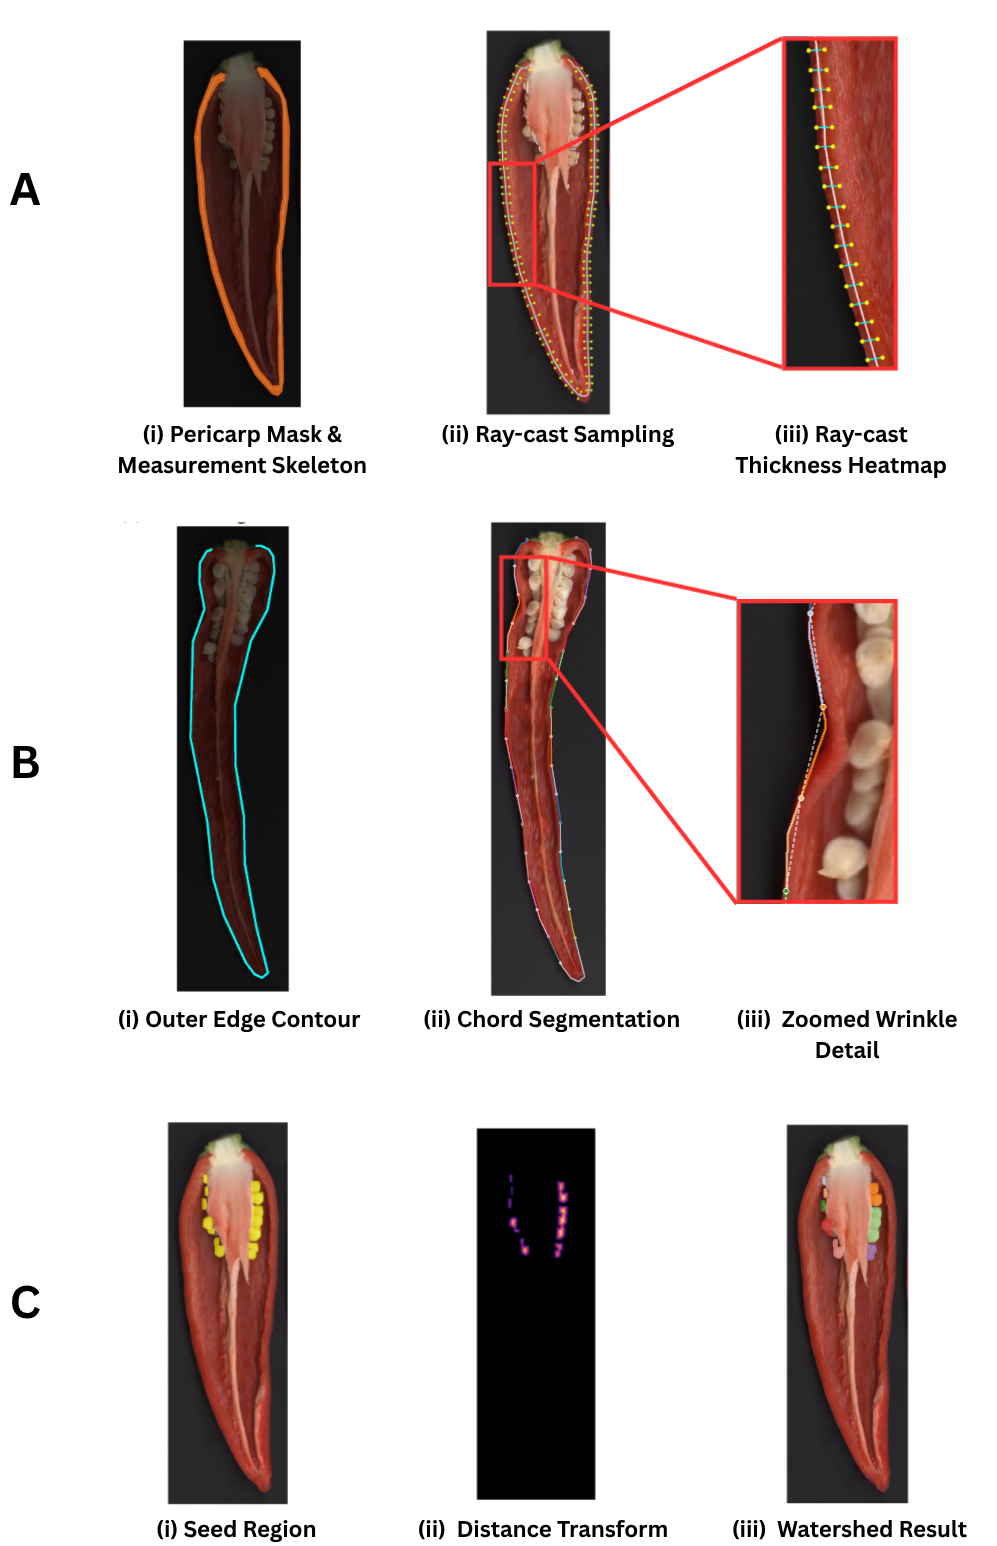
\includegraphics[width=0.9\linewidth,height=0.48\textheight,keepaspectratio]{images/pedicel_placeholder.png}
\caption[Pedicel separation illustration (draft)]{\textbf{Draft placeholder for the mask-processing illustration.} Planned panel (A): pedicel separation from the PCP mask. Panels (B) and (C): to be determined. The image is temporarily copied from Fig.~\ref{fig:method_thickness_wrinkle_seed} and does not yet illustrate the planned panels.}
\label{fig:pedicel_separation}
\end{figure}

\begin{figure}[htbp]
\centering
% Replace with your actual image path
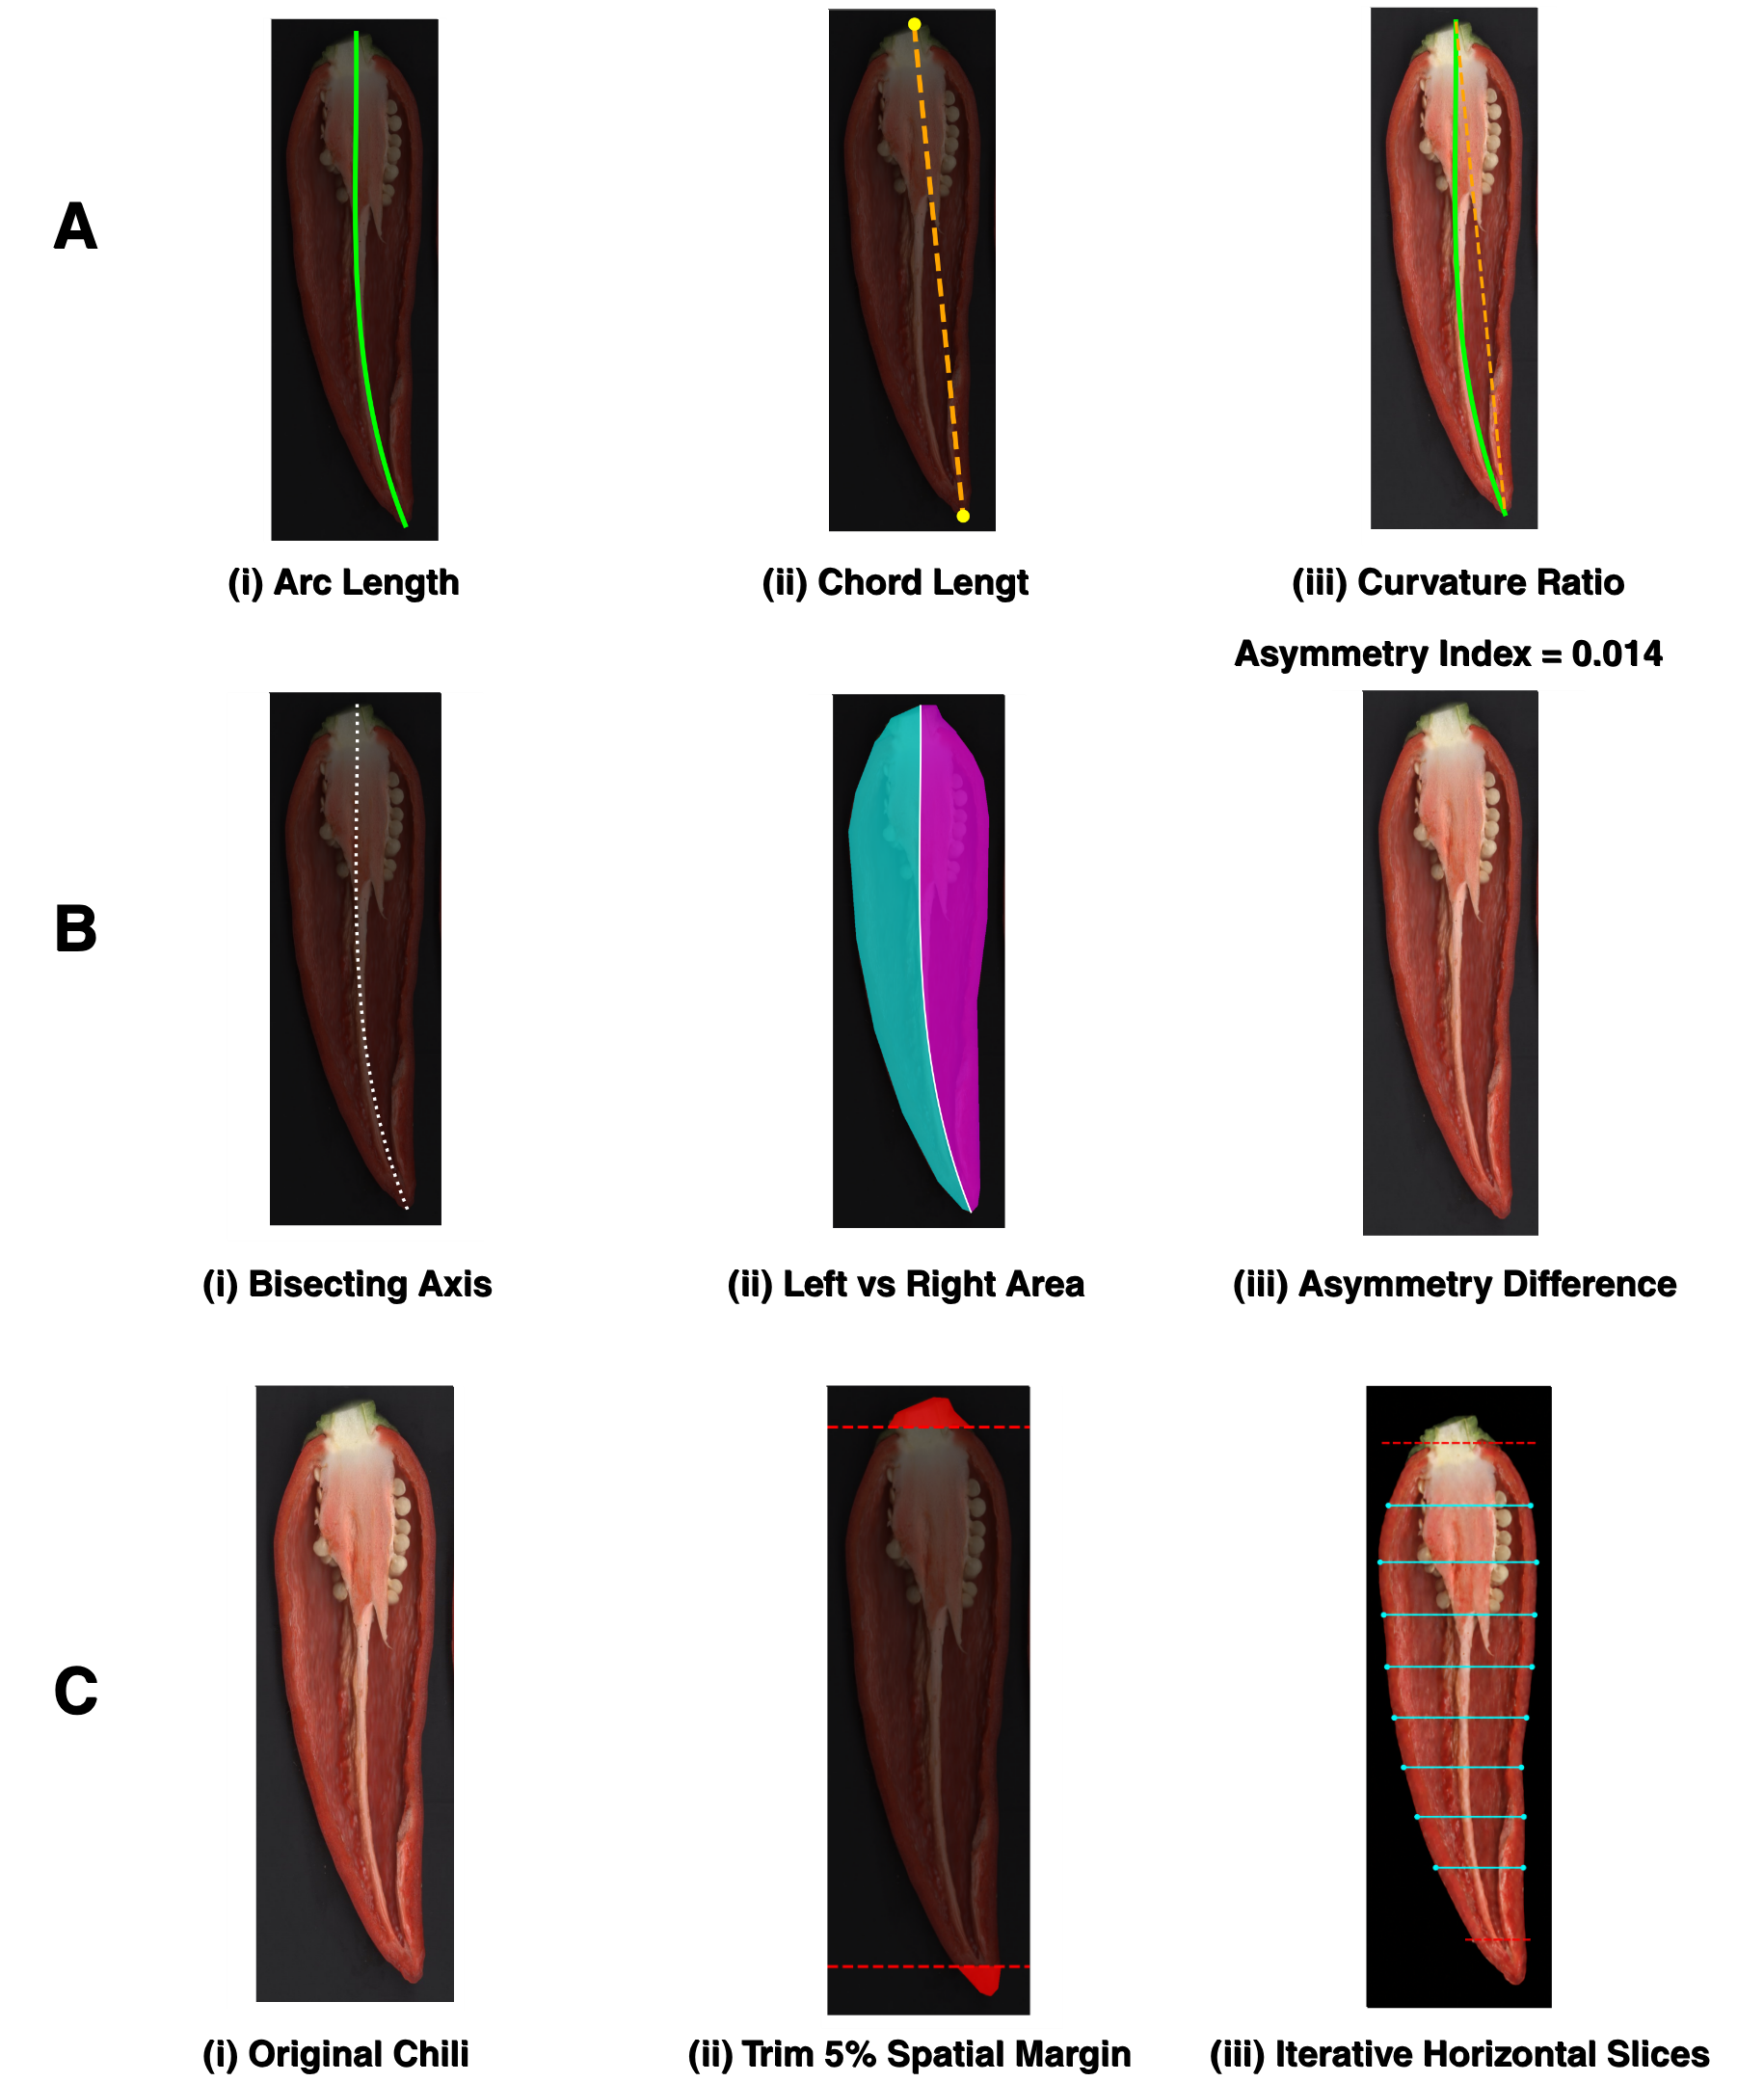
\includegraphics[width=0.9\linewidth]{images/fig_1.png}
\caption{\textbf{Geometric feature extraction for fruit curvature, fruit asymmetry, and mean fruit width.} (A) The Fruit Curvature Index ($FCI$) captures global bending as one minus the regularized ratio of the endpoint chord length to the fitted fruit-body spine length; values near zero indicate a nearly straight axis, and larger values indicate greater bending. (B) Left and right widths are compared relative to the straight line joining the endpoints of the fitted fruit-body spine to derive maximum leftward, maximum rightward, and mean signed deviation. (C) Mean Fruit Width ($FW_{\mathrm{mean}}$) is calculated as the average of eight horizontal chords measured at the interior scanlines among ten equally spaced scanlines spanning the fruit-mask extent.}
\label{fig:method_curvature_asym_width}
\end{figure}

\subsection*{Extract Fruit Area ($FA$)}

Fruit area ($FA$) is measured on the fruit-body mask, obtained by removing the outer region and the separated pedicel from the whole-fruit mask:

\begin{equation}
M_{\mathrm{body}}=M_{\mathrm{chili}}\setminus\left(M_{\mathrm{pedicel}}\cup M_{\mathrm{outer}}\right).
\end{equation}

Here, $M_{\mathrm{body}}$ is the binary fruit-body mask. Fruit area is calculated as:

\begin{equation}
FA=\gamma^2|M_{\mathrm{body}}|.
\end{equation}

Here, $FA$ is Fruit Area in mm$^2$. Throughout the mask-area formulas, $|M|$ denotes the number of foreground pixels belonging to the binary mask $M$ (pixels with nonzero mask values). Thus, $|M_{\mathrm{body}}|$ counts the pixels in the fruit-body mask. Multiplication by $\gamma^2$ converts this pixel count to area in mm$^2$.

\subsection*{Extraction of Fruit Length ($FL$) and Fruit Width ($FW$)}

The fitted central spine used for fruit-length estimation is illustrated in Fig.~\ref{fig:method_curvature_asym_width}A. Fruit length is estimated from a central spine fitted to the previously defined fruit-body mask $M_{\mathrm{body}}$.

For each nonempty image row of $M_{\mathrm{body}}$, the midpoint between the leftmost and rightmost foreground pixels is calculated. A third-degree polynomial, $x=f_3(y)$, is fitted to these midpoints, where $y$ is the image-row coordinate and $f_3(y)$ gives the horizontal coordinate of the fitted central spine at that row. The spine arc length is approximated by a discrete sum over the valid pixel rows:

\begin{equation}
 FL\approx\gamma\sum_{y\in\mathcal{Y}_{\mathrm{spine}}}\sqrt{1+\left[f'_3(y)\right]^2}\,\Delta y,\qquad\Delta y=1\text{ pixel}.
\end{equation}
Here, $\mathcal{Y}_{\mathrm{spine}}$ is the set of nonempty rows of $M_{\mathrm{body}}$ and $f'_3(y)$ is the first derivative of the fitted polynomial. Fruit length is rounded to two decimal places.

The horizontal scanlines used for fruit-width measurement are illustrated in Fig.~\ref{fig:method_curvature_asym_width}C. Fruit width is measured directly from the fruit mask using horizontal
scanlines. Ten equally spaced scanlines span the mask's occupied vertical
extent, dividing it into nine equal intervals:
\begin{equation}
    y_k = \operatorname{round}\left(
    y_{\min}^{\mathrm{mask}} +
    \frac{k}{9}\left(y_{\max}^{\mathrm{mask}}-y_{\min}^{\mathrm{mask}}\right)
    \right), \qquad k=0,\ldots,9.
\end{equation}
Here, $y_{\min}^{\mathrm{mask}}$ and $y_{\max}^{\mathrm{mask}}$ are the topmost and bottommost image-row coordinates occupied by the fruit mask, respectively; $y_k$ is the row coordinate of scanline $k$, and $\operatorname{round}$ rounds to the nearest integer pixel row.

The two endpoint scanlines are excluded. At each of the eight interior
scanlines, $k=1,\ldots,8$, the horizontal chord extends from the leftmost
to the rightmost foreground pixel of the fruit mask. Its physical width is
\begin{equation}
    FW_k = \gamma\left(x_{\mathrm{right}}(y_k)
    - x_{\mathrm{left}}(y_k)\right).
\end{equation}
Here, $x_{\mathrm{left}}(y_k)$ and $x_{\mathrm{right}}(y_k)$ are the horizontal pixel coordinates of the leftmost and rightmost foreground pixels at row $y_k$, respectively, and $FW_k$ is the corresponding fruit width in mm.

The minimum, mean, and maximum fruit widths are calculated from these eight
measurements:
\begin{align}
    FW_{\min} &= \min_{k=1,\ldots,8} FW_k, \\
    FW_{\mathrm{mean}} &= \frac{1}{8}\sum_{k=1}^{8} FW_k, \\
    FW_{\max} &= \max_{k=1,\ldots,8} FW_k.
\end{align}
Here, $FW_{\min}$, $FW_{\mathrm{mean}}$, and $FW_{\max}$ are the minimum, mean, and maximum fruit widths measured at the eight interior scanlines, respectively, all in mm.


\subsection*{Extract Fruit Curvature Index ($FCI$)}
The Fruit Curvature Index ($FCI$) describes the overall bending of the fruit body through the relationship between the straight-line distance connecting the spine endpoints and the spine length. It uses the spine $x=f_3(y)$ fitted to $M_{\mathrm{body}}$ during fruit-length estimation, as illustrated in Fig.~\ref{fig:method_curvature_asym_width}A:

\begin{equation}
 FCI=1-\frac{\varepsilon_{\mathrm{C}}+\gamma\sqrt{[f_3(y_{\max})-f_3(y_{\min})]^2+(y_{\max}-y_{\min})^2}}{\varepsilon_{\mathrm{C}}+FL}.
\end{equation}
Here, $y_{\min}$ and $y_{\max}$ are the first and last row coordinates of the fruit-body spine, respectively; $\varepsilon_{\mathrm{C}}=10^{-6}\,\mathrm{mm}$ is a small positive constant that prevents a zero denominator. The square-root expression multiplied by $\gamma$ gives the straight-line distance between the spine endpoints. FCI values near zero indicate a nearly straight spine, whereas values closer to one indicate greater overall bending.

\subsection*{Extraction of Deviation}

Left--right deviation of the fruit body is determined by comparing the widths on either side of a common reference line, as illustrated in Fig.~\ref{fig:method_curvature_asym_width}B. Let $x=f_{\mathrm{axis}}(y)$ denote the straight line joining the endpoints of the spine $x=f_3(y)$ fitted to $M_{\mathrm{body}}$ during fruit-length and curvature estimation. At each row $y\in\mathcal{Y}_{\mathrm{spine}}$, the dividing position is constrained to lie between the two boundaries:

\begin{equation}
\tilde{x}(y)=\min\!\left[x_{\mathrm{right}}(y),\,\max\!\left(x_{\mathrm{left}}(y),f_{\mathrm{axis}}(y)\right)\right].
\end{equation}

Here, $\tilde{x}(y)$ is the constrained horizontal dividing coordinate; the boundary coordinates in this step are taken from $M_{\mathrm{body}}$. The left and right widths are calculated as:

\begin{equation}
W_L(y)=\tilde{x}(y)-x_{\mathrm{left}}(y),\qquad W_R(y)=x_{\mathrm{right}}(y)-\tilde{x}(y).
\end{equation}

Here, $W_L(y)$ and $W_R(y)$ are the widths of the fruit body to the left and right of the reference line at row $y$, respectively, in pixels. When the reference line lies outside the boundary span, the full row width is assigned to the side containing the fruit, while the opposite side has zero width. Signed row-wise deviation is normalized by the total width:

\begin{equation}
d(y)=\frac{W_R(y)-W_L(y)}{W_R(y)+W_L(y)+\varepsilon_{\mathrm{A}}},\qquad y\in\mathcal{Y}_{\mathrm{spine}}.
\end{equation}

Here, $\varepsilon_{\mathrm{A}}=10^{-6}\,\mathrm{pixel}$ is a small positive constant that prevents a zero denominator; a zero-width row therefore has $d(y)=0$. Negative values indicate leftward deviation, positive values indicate rightward deviation, and zero indicates equal widths on both sides. Since $\varepsilon_{\mathrm{A}}>0$, $d(y)\in(-1,1)$; values approach $-1$ or $1$ when the entire row width lies to the left or right of the reference line, respectively. The maximum leftward deviation ($D_L$), maximum rightward deviation ($D_R$), and mean signed deviation ($D_{\mathrm{mean}}$) are calculated as:

\begin{equation}
D_L=\min\!\left(0,\min_{y\in\mathcal{Y}_{\mathrm{spine}}}d(y)\right).
\end{equation}

\begin{equation}
D_R=\max\!\left(0,\max_{y\in\mathcal{Y}_{\mathrm{spine}}}d(y)\right).
\end{equation}

\begin{equation}
D_{\mathrm{mean}}=\frac{1}{|\mathcal{Y}_{\mathrm{spine}}|}\sum_{y\in\mathcal{Y}_{\mathrm{spine}}}d(y).
\end{equation}

Here, $|\mathcal{Y}_{\mathrm{spine}}|$ denotes the number of valid image rows. $D_{\mathrm{mean}}$ is calculated by summing the signed deviations $d(y)$ over these rows and dividing by their number. All three indices are dimensionless. $D_L\in(-1,0]$ and $D_R\in[0,1)$ describe the strongest deviation toward each side; zero indicates that no row deviates toward that side. $D_{\mathrm{mean}}\in(-1,1)$ describes the overall directional tendency, with equal weight assigned to each row. A mean near zero does not necessarily imply a symmetric fruit body, because leftward and rightward deviations can cancel.

\subsection*{Extract Mesocarp Area ($MA$)}

To construct the mesocarp mask, the outer mask is first subtracted from the whole-fruit mask. The resulting mask is cleaned by morphological opening and connected-component filtering before the internal anatomical masks are removed. A final component filter suppresses small isolated remnants. Denoting these two cleaning operations by $\mathcal{C}$ and $\mathcal{F}$, respectively, the runtime mask can be written as
\begin{equation}
 M_{\mathrm{mesocarp}}=\mathcal{F}\!\left[\mathcal{C}(M_{\mathrm{chili}}\setminus M_{\mathrm{outer}})\setminus\left(M_{\mathrm{endocarp}}\cup M_{\mathrm{PCP}}\cup M_{\mathrm{seed}}\right)\right].
\end{equation}
The mesocarp area ($MA$) is therefore:
\begin{equation}
    MA=\gamma^2|M_{\mathrm{mesocarp}}|.
\end{equation}
Here, $MA$ is Mesocarp Area in mm$^2$, and $|M_{\mathrm{mesocarp}}|$ is the number of foreground pixels belonging to the retained mesocarp mask.

\subsection*{Extract Mesocarp Thickness}

The mesocarp mask $M_{\mathrm{mesocarp}}$ is additionally smoothed using morphological operations to reduce small boundary irregularities and skeleton branches caused by segmentation noise. The smoothed mask is used consistently to determine the inner and outer boundaries and construct the skeleton for thickness measurement.

The skeleton represents the medial axis of the mesocarp region. Side branches are removed by retaining the longest geodesic backbone in each skeleton component. Measurement locations $\mathbf{s}_i$ are sampled along the skeleton at an arc-length interval of $1\,\mathrm{mm}$ to distribute measurements along the tissue.

At each location $\mathbf{s}_i$, straight lines passing through the point are examined in multiple directions. A measurement line is valid when it intersects the inner and outer boundaries on opposite sides of $\mathbf{s}_i$. Among the valid measurement segments, the shortest segment connecting the two intersections is selected as the local mesocarp thickness, as illustrated in Fig.~\ref{fig:method_thickness_wrinkle_seed}A:

\begin{equation}
T_i=\gamma\min_{\theta\in\Theta}\left\|\mathbf{p}^{\,\mathrm{inner}}_{i,\theta}-\mathbf{p}^{\,\mathrm{outer}}_{i,\theta}\right\|_2.
\end{equation}

Here, $T_i$ is the thickness at location $\mathbf{s}_i$ in mm; $\theta$ is the measurement-line angle and $\Theta$ is the set of surveyed directions. The points $\mathbf{p}^{\,\mathrm{inner}}_{i,\theta}$ and $\mathbf{p}^{\,\mathrm{outer}}_{i,\theta}$ are the intersections of the measurement line with the inner and outer boundaries of the smoothed mesocarp mask, respectively. The notation $\|\cdot\|_2$ denotes the Euclidean distance between the two intersections. The minimum is evaluated over the surveyed directions that yield valid measurement segments.

Let $\mathcal{T}$ denote the collection of successfully obtained local thickness measurements. The minimum, mean, and maximum mesocarp thicknesses are calculated as:

\begin{align}
MT_{\min} &= \min_{T_i\in\mathcal{T}}T_i,\\
MT_{\mathrm{mean}} &= \frac{1}{|\mathcal{T}|}\sum_{T_i\in\mathcal{T}}T_i,\\
MT_{\max} &= \max_{T_i\in\mathcal{T}}T_i.
\end{align}

Here, $|\mathcal{T}|$ is the number of measurements used. $MT_{\min}$, $MT_{\mathrm{mean}}$, and $MT_{\max}$ represent the minimum, mean, and maximum thicknesses at the measured locations, respectively, all in mm.

\subsection*{Extract Placenta Area ($PA$)}
The placenta area ($PA$) is computed directly from the placenta mask obtained after pedicel separation:
\begin{equation}
 PA=\gamma^2|M_{\mathrm{placenta}}|.
\end{equation}
Here, $|M_{\mathrm{placenta}}|$ is the number of foreground pixels in the placenta mask.

\subsection*{Extract Mesocarp Area Fraction ($MAF$)}

Mesocarp Area Fraction ($MAF$) measures the proportion of the fruit-body cross-section occupied by mesocarp. Using the previously defined fruit area $FA$, the fraction is calculated from unrounded areas as:

\begin{equation}
 MAF=\frac{|M_{\mathrm{mesocarp}}|}{|M_{\mathrm{body}}|}=\frac{MA^*}{FA^*},
\end{equation}
where $|M_{\mathrm{mesocarp}}|$ and $|M_{\mathrm{body}}|$ count the foreground pixels in the mesocarp and fruit-body masks, respectively; $MA^*$ and $FA^*$ denote the corresponding physical areas before rounding for display. The common spatial calibration factor cancels. For valid masks, $MAF\in[0,1]$.


\subsection*{Extract Mesocarp Wrinkle Index ($MWI$)}

The Mesocarp Wrinkle Index ($MWI$) is determined from the tortuosity of the external contour of the fruit-body mask $M_{\mathrm{body}}$, as illustrated in Fig.~\ref{fig:method_thickness_wrinkle_seed}B. The contour is divided into consecutive segments using a chord-length threshold of $\tau=5\,\mathrm{mm}$, corresponding to $\tau_{\mathrm{px}}=\tau/\gamma$ pixels. From the start of each segment, the algorithm traverses the contour to the first point whose straight-line distance from the start reaches this threshold. The endpoint is interpolated on the contour and used as the start of the next segment.

For each segment $i$, let $L_{\mathrm{arc},i}$ denote the length measured along the contour and $L_{\mathrm{chord},i}$ the straight-line distance between its endpoints. The wrinkle index is the mean relative difference between these lengths:

\begin{equation}
MWI=\frac{1}{N}\sum_{i=1}^{N}\left(1-\frac{L_{\mathrm{chord},i}}{L_{\mathrm{arc},i}}\right).
\end{equation}

Here, $N$ is the number of valid segments with positive arc and chord lengths; $L_{\mathrm{arc},i}$ and $L_{\mathrm{chord},i}$ are expressed in the same length units. Each segment has equal weight in the mean. MWI is dimensionless and lies in $[0,1)$. Values near zero indicate nearly straight contour segments, whereas values closer to one indicate greater tortuosity. The measurement describes fruit-body contour irregularity at the selected chord scale, including contributions from both corrugation and local curvature.

\subsection*{Extract Total Seed Area ($SA$) and Seed Count ($SC$)}
The seeds are identified directly from YOLO-predicted instance masks of the seed class. After confidence filtering and clipping to the fruit region, each nonempty mask is treated as one seed. Let $N_s$ be the number of retained seed instances and $M_{\mathrm{seed},j}$ the binary mask of seed $j$. The combined seed mask is the union of these instance masks:

\begin{equation}
M_{\mathrm{seed}}=\bigcup_{j=1}^{N_s}M_{\mathrm{seed},j}.
\end{equation}
The total seed area is calculated from this union mask, while seed count is obtained directly from the retained YOLO instances:

\begin{align}
SA&=\gamma^2|M_{\mathrm{seed}}|,\\
SC&=N_s.
\end{align}
Here, $|M_{\mathrm{seed}}|$ is the number of foreground pixels in the union seed mask, $SA$ is expressed in mm$^2$, and $SC$ is the number of detected seeds. Each pixel in the union mask contributes to $SA$ only once, including pixels shared by multiple seed instances. Overlapping instances remain separate seeds for $SC$. When no seed instances are retained, $M_{\mathrm{seed}}$ is empty and $SA=SC=0$.


\subsection*{Extract Seed-to-Cavity Area Ratio ($SCR$)}
The Seed-to-Cavity Area Ratio ($SCR$) uses the area of the union seed mask, which counts each covered pixel once. Let $M_{\mathrm{cavity}}=M_{\mathrm{endocarp}}$. The runtime computes
\begin{equation}
 SCR=\frac{|M_{\mathrm{seed}}|}{|M_{\mathrm{endocarp}}|+\varepsilon_{\mathrm{SCR}}}.
\end{equation}
Here, $|M_{\mathrm{seed}}|$ and $|M_{\mathrm{endocarp}}|$ are the numbers of foreground pixels in the union seed mask and the current endocarp mask, respectively. The small positive constant $\varepsilon_{\mathrm{SCR}}=10^{-6}$ is specified in pixel-count units and prevents a zero denominator. It is distinct from $\varepsilon_{\mathrm{C}}$ and $\varepsilon_{\mathrm{A}}$ used above. $SCR$ is dimensionless. Before display rounding, it lies in $[0,1)$ when the seed mask is contained in the endocarp mask. It is zero for an empty seed mask; an empty endocarp mask with detected seed pixels yields a large finite value. Its numerator equals $SA/\gamma^2$ before rounding $SA$ for display, because both measurements use the same union seed mask.

\subsection*{Extract Redness}
Redness is measured over the fruit region after removing the seed, outer, and PCP masks:

\begin{equation}
M_{\mathrm{color}}=M_{\mathrm{chili}}\setminus\left(M_{\mathrm{seed}}\cup M_{\mathrm{outer}}\cup M_{\mathrm{PCP}}\right).
\end{equation}
The RGB image is converted to CIELAB. The value $a^*(x,y)$ represents the coordinate along the green--red axis at pixel $(x,y)$ and is recovered by subtracting 128 from the $a$ channel of the 8-bit OpenCV Lab image \cite{cielab}. For $|M_{\mathrm{color}}|>0$, mean redness is calculated as:

\begin{equation}
R=\frac{1}{|M_{\mathrm{color}}|}\sum_{(x,y)\in M_{\mathrm{color}}}a^*(x,y).
\end{equation}
Here, $|M_{\mathrm{color}}|$ is the number of foreground pixels in the measurement region. Higher $R$ values indicate a stronger tendency toward red, whereas negative values indicate a tendency toward green. The endocarp mask is not separately excluded, so endocarp pixels remaining after mask subtraction are included in the measurement.

This index describes color in the selected image region and is not treated as a direct measurement of ripeness. When the measurement region is empty, the runtime returns zero and marks the color measurement as unavailable.


\begin{figure}[htbp]
\centering
% Replace with your actual image path
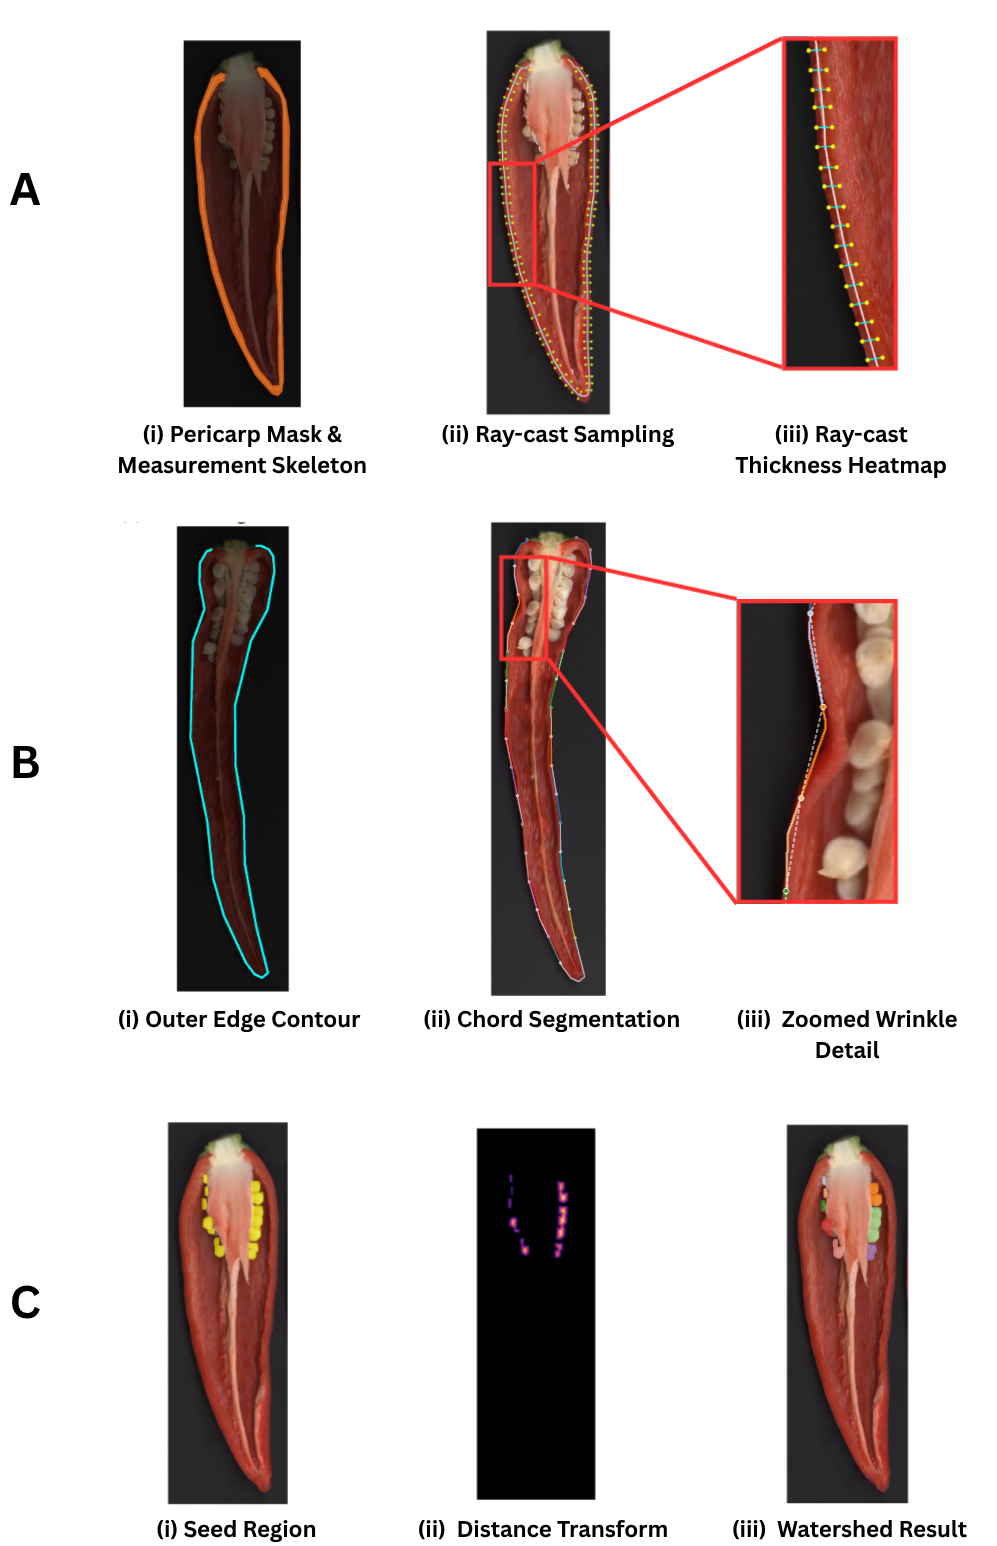
\includegraphics[width=0.9\linewidth]{images/fig_2.png}
\caption{\textbf{Extraction of mesocarp thickness, fruit-body contour irregularity, and seed count.} (A) Mesocarp thickness is estimated at sampled skeleton locations by selecting the shortest valid line through each location that intersects the inner and outer mesocarp boundaries. (B) Contour irregularity is summarized by the mean of one minus the chord-to-arc length ratio on the external contour of the fruit-body mask, using a 5 mm chord threshold. (C) The earlier watershed seed-separation workflow is shown for comparison; the present $SA$ and $SC$ measurements use YOLO seed instance masks.}
\label{fig:method_thickness_wrinkle_seed}
\end{figure}

\section{Results}

\subsection{Instance Segmentation Performance}

\begin{table*}[htbp]
\centering
\caption{Comparison of YOLO instance-segmentation models on the accession-held-out test set at an input resolution of \texttt{imgsz=960}. Metrics are macro-averaged over the four reported anatomical classes: seed, outer, placenta, and endocarp.}
\label{tab:model_comparison}
\begin{tabular}{lcccc}
\hline
Model & Precision (\%) & Recall (\%) & mAP@0.5 (\%) & mAP@0.5:0.95 (\%) \\
\hline
YOLOv8s-seg & 88.78 & 79.75 & 85.01 & 45.22 \\
YOLOv8m-seg & 86.53 & 82.77 & 85.74 & 46.47 \\
YOLO11s-seg & 85.74 & 82.63 & 84.05 & 45.15 \\
YOLO11m-seg & 84.31 & 84.18 & 84.99 & 45.88 \\
YOLO26s-seg & 83.14 & 78.79 & 80.44 & 42.84 \\
YOLO26m-seg & 86.36 & 77.80 & 81.26 & 43.33 \\
\hline
\end{tabular}
\end{table*}

Table~\ref{tab:model_comparison} reports mask-based Precision, Recall, mAP@0.5, and mAP@0.5:0.95, macro-averaged over the four anatomical classes, for six candidate architectures evaluated on the accession-held-out test set. YOLOv8m-seg achieved the highest mask mAP@0.5 (85.74\%) among the six evaluated models. Its mask mAP@0.5:0.95 was 46.47\%. YOLOv8m-seg was selected as the final backbone based on its highest mAP@0.5 and moderate computational cost. Per-class results are reported in Table~\ref{tab:per_class}.

\begin{table}[htbp]
\centering
\caption{Per-class mask-segmentation performance of the selected YOLOv8m-seg model at \texttt{imgsz=960} on the accession-held-out test set. The composite placenta--pedicel class is denoted PCP in the runtime implementation and ``placenta'' in the evaluation files.}
\label{tab:per_class}
\begin{tabular}{lccccc}
\hline
Class & Precision (\%) & Recall (\%) & F1-score (\%) & mAP@0.5 (\%) & mAP@0.5:0.95 (\%) \\
\hline
Seed & 94.48 & 92.62 & 93.54 & 95.37 & 53.81 \\
Outer & 83.15 & 70.89 & 76.53 & 85.85 & 51.18 \\
PCP (placenta--pedicel) & 90.99 & 89.64 & 90.31 & 93.83 & 62.59 \\
Endocarp & 77.51 & 77.95 & 77.73 & 67.93 & 18.32 \\
\hline
\end{tabular}
\end{table}

\subsection{Phenotypic Trait Extraction Results}

\begin{table*}[htbp]
\centering
\footnotesize
\caption{Descriptive statistics of selected phenotypic traits calculated from 264 individual chili-fruit crops. Each crop contributes one fruit-level observation; the 367 images reported for the full dataset refer to original multi-fruit images. CV denotes the coefficient of variation (SD/mean $\times100$).}
\label{tab:descriptive_stats}
\resizebox{\textwidth}{!}{
\begin{tabular}{llcccc}
\hline
\textbf{Domain} & \textbf{Trait} & \textbf{Unit} & \textbf{Mean $\pm$ SD} & \textbf{Min -- Max} & \textbf{CV (\%)} \\
\hline
\multirow{8}{*}{Size \& Geometric}
 & Fruit Length ($FL$) & mm & 105.00 $\pm$ 38.10 & 26.06 -- 221.64 & 36.3 \\
 & Mean Fruit Width ($FW_{mean}$) & mm & 23.05 $\pm$ 16.30 & 7.17 -- 76.23 & 70.7 \\
 & Minimum Fruit Width ($FW_{min}$) & mm & 14.41 $\pm$ 11.16 & 3.79 -- 60.10 & 77.5 \\
 & Maximum Fruit Width ($FW_{max}$) & mm & 28.06 $\pm$ 19.16 & 9.34 -- 85.09 & 68.3 \\
 & Fruit Area ($FA$) & mm$^2$ & 2320.47 $\pm$ 2018.59 & 281.47 -- 11151.25 & 87.0 \\
 & Mesocarp Area ($MA$) & mm$^2$ & 565.03 $\pm$ 522.52 & 68.93 -- 2666.87 & 92.5 \\
 & Mean Mesocarp Thickness ($MT_{mean}$) & mm & 2.50 $\pm$ 1.93 & 0.77 -- 8.51 & 77.1 \\
 & Maximum Mesocarp Thickness ($MT_{max}$) & mm & 4.66 $\pm$ 3.70 & 1.15 -- 15.80 & 79.3 \\
\hline
\multirow{4}{*}{Internal Anatomical \& Seed}
 & Placenta Area ($PA$) & mm$^2$ & 420.01 $\pm$ 338.79 & 52.16 -- 1861.93 & 80.7 \\
 & Mesocarp Area Fraction ($MAF$) & -- & 0.25 $\pm$ 0.05 & 0.15 -- 0.42 & 20.1 \\
 & Seed Count ($SC$) & seed & 11.94 $\pm$ 8.11 & 0.00 -- 40.00 & 67.9 \\
 & Seed-to-Cavity Area Ratio ($SCR$) & -- & 0.11 $\pm$ 0.08 & 0.00 -- 0.44 & 73.9 \\
\hline
\multirow{4}{*}{Shape \& Colorimetric}
 & Fruit Curvature Index ($FCI$) & -- & 0.99 $\pm$ 0.02 & 0.89 -- 1.00 & 1.8 \\
 & Fruit Asymmetry Index ($FAI$) & -- & 0.05 $\pm$ 0.03 & 0.01 -- 0.21 & 67.1 \\
 & Mesocarp Wrinkle Index ($MWI$) & -- & 0.15 $\pm$ 0.18 & 0.04 -- 1.23 & 119.2 \\
 & Redness & -- & 33.51 $\pm$ 4.32 & 12.66 -- 40.53 & 12.9 \\
\hline
\end{tabular}
}
\end{table*}


Table~\ref{tab:descriptive_stats} summarizes the selected traits for the 264 fruit cross-sections included in this analysis. Fruit Length ($FL$) had a mean of 105.00 mm and a coefficient of variation of 36.3\%. Mesocarp Area Fraction ($MAF$) had a mean of 0.25 and a coefficient of variation of 20.1\%. These descriptive statistics are calculated at the individual fruit level.

To assess measurement reliability in the absence of a manual reference for morphologically derived traits (e.g., $FCI$, $FAI$, and $SCR$), we quantified the proportion of total trait variance attributable to between-variety differences relative to within-variety (biological/measurement) variance using one-way ANOVA grouped by accession ($\eta^2$). Fruit Length ($FL$) and Mean Fruit Width ($FW_{\mathrm{mean}}$) exhibited a between-variety variance ratio of 98.2\% and 99.1\%, respectively, indicating that between-accession differences account for a large share of their observed variation. The advanced algorithmic traits introduced in this study likewise showed a substantial between-variety component: $FAI$ ($\eta^2=77.8\%$), $SCR$ ($\eta^2=64.4\%$), and $FCI$ ($\eta^2=54.0\%$). These results indicate substantial between-accession variation in the examined traits. However, this analysis does not distinguish measurement error from biological variation within accessions; independent reference measurements would be needed to assess measurement accuracy.

As an exploratory biological check using the 264 fruit-level observations summarized in Table~\ref{tab:descriptive_stats}, seed count and fruit-body area showed a positive Pearson correlation ($r=0.336$, $p=2.18\times10^{-8}$). After averaging both traits within each accession, the correlation was $r=0.426$ ($p=0.00494$; $n=42$ accessions). These associations describe phenotypic covariation and do not independently validate seed-count accuracy.

\begin{figure}[htbp]
\centering
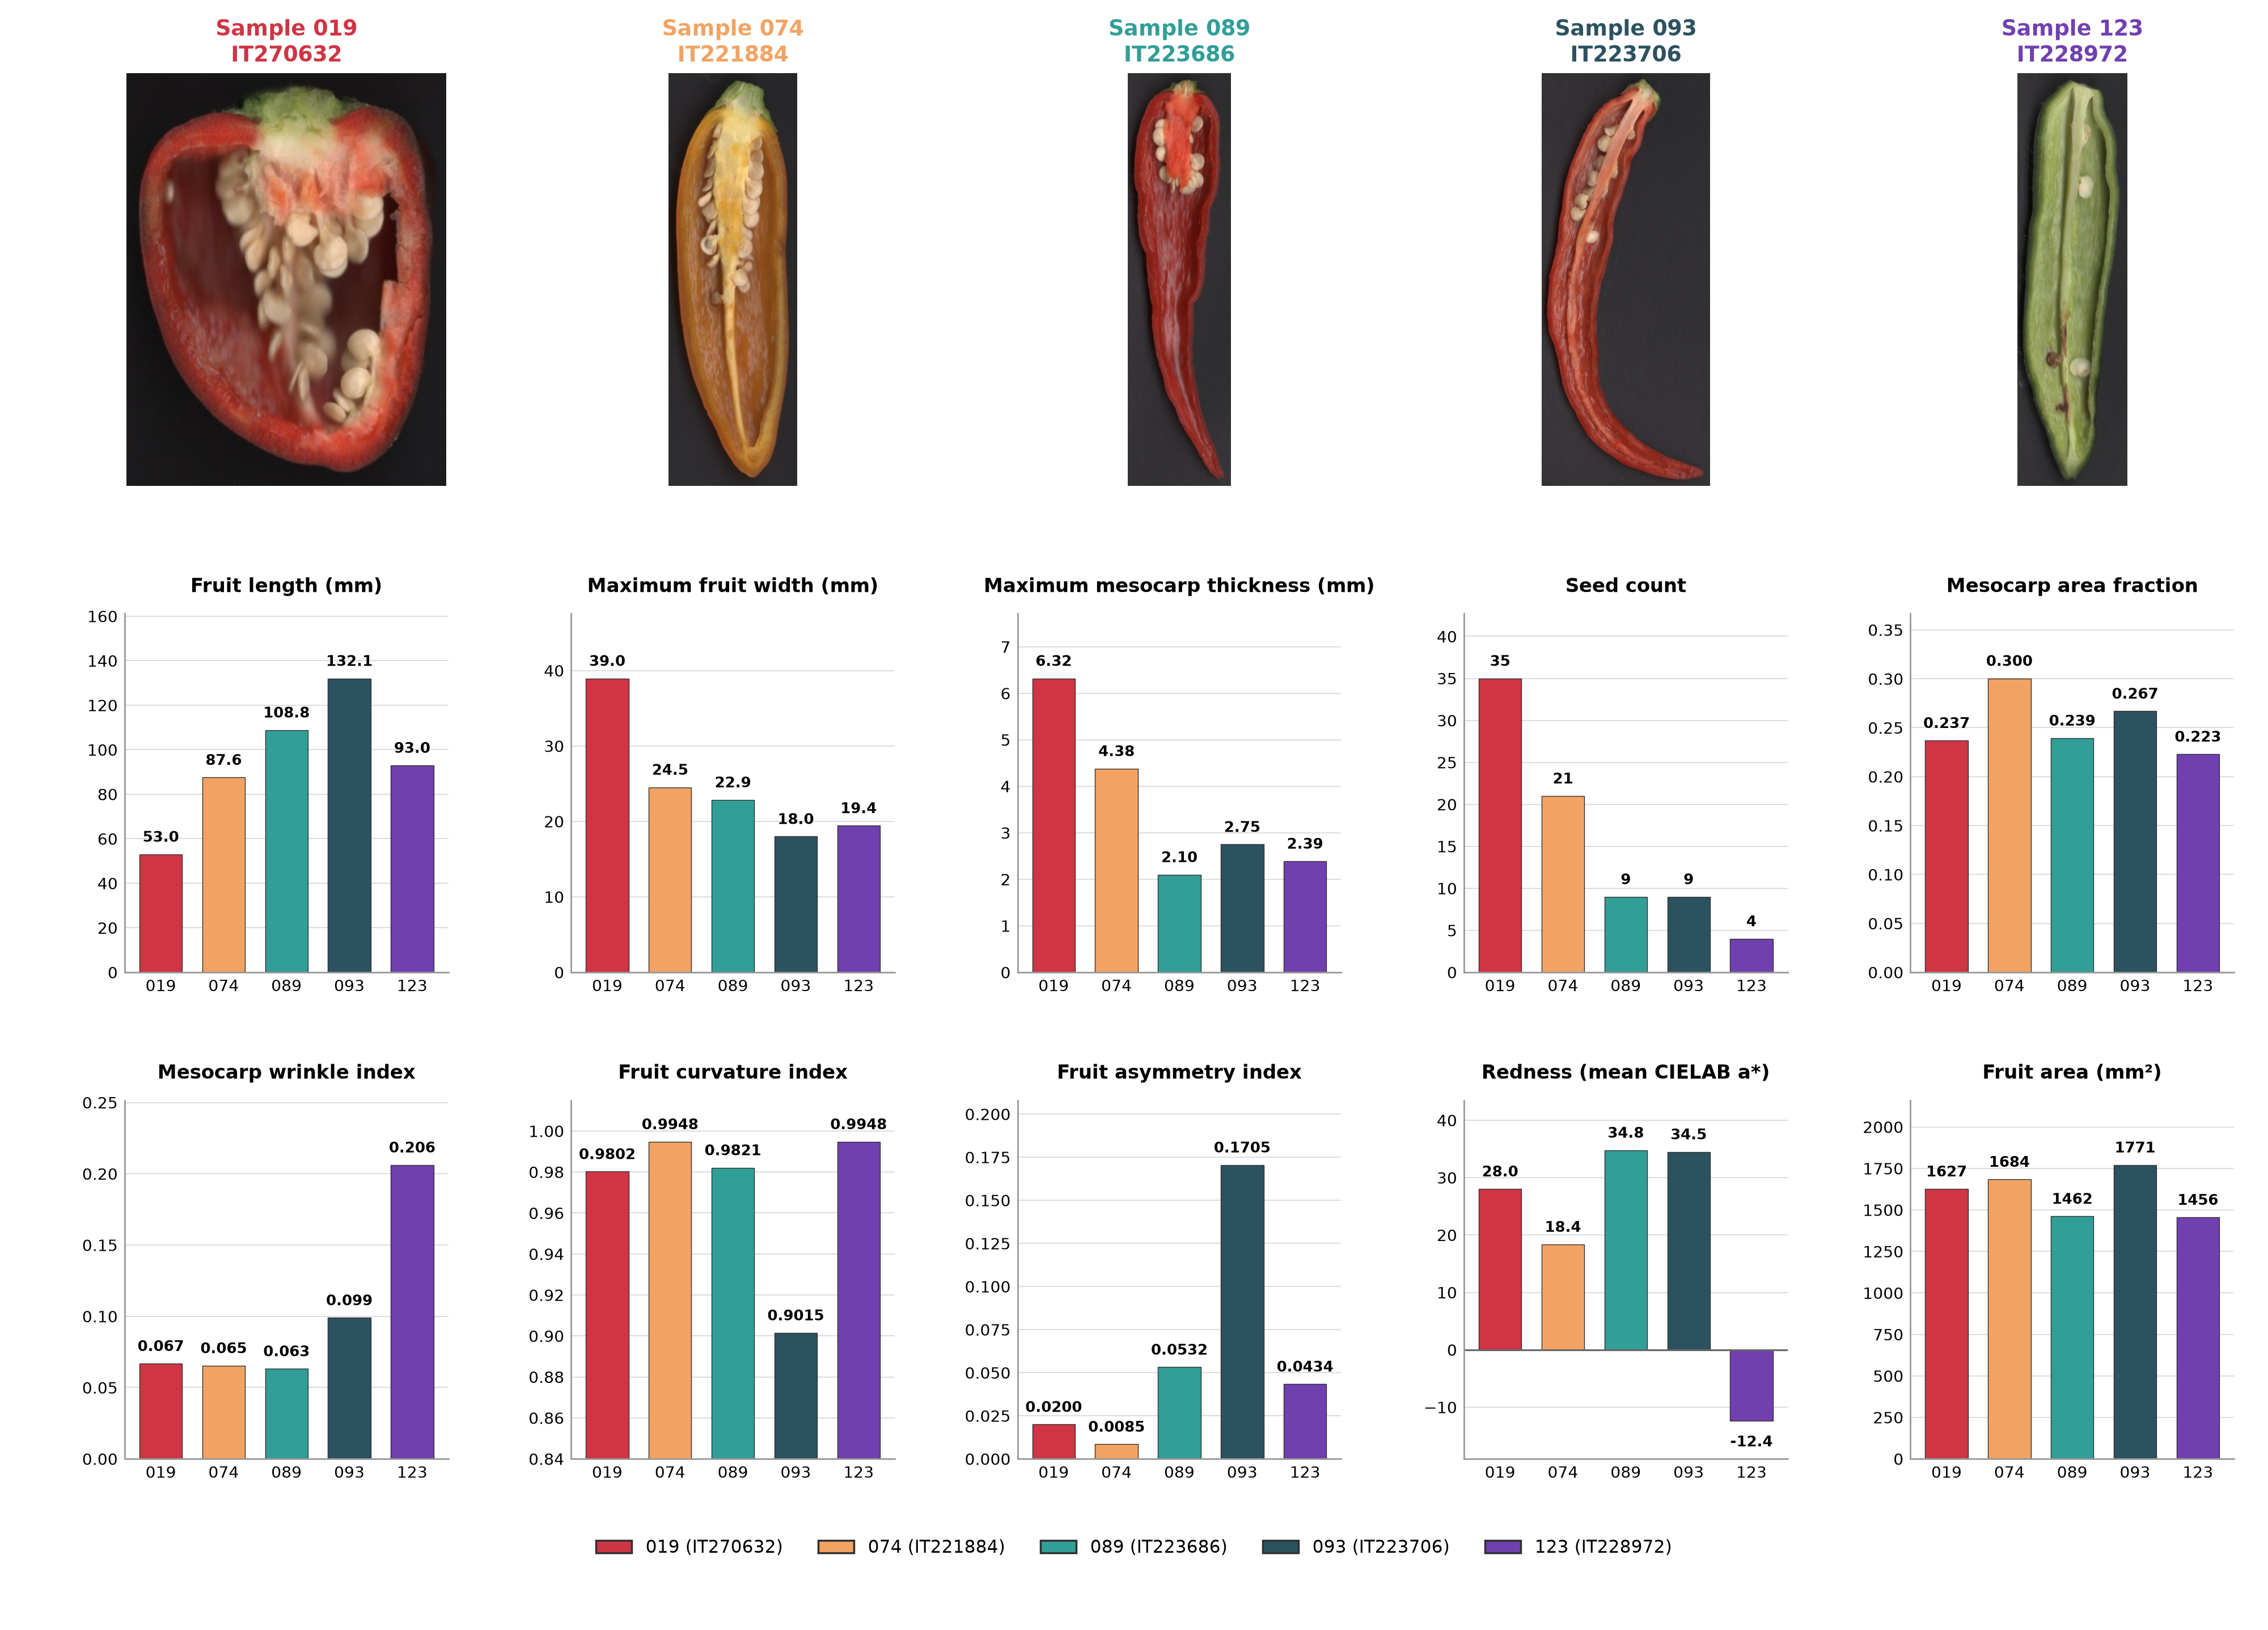
\includegraphics[width=0.85\linewidth]{images/Sample.png}
\caption{\textbf{Automated phenotyping of five example longitudinally sectioned chili fruits.} The images show the leftmost fruit from images 019 (IT270632), 074 (IT221884), 089 (IT223686), 093 (IT223706), and 123 (IT228972); each image is cropped and scaled independently for display. From left to right, the bar-chart panels report Fruit Length ($FL$), Maximum Fruit Width ($FW_{\max}$), Maximum Mesocarp Thickness ($MT_{\max}$), Seed Count ($SC$), Mesocarp Area Fraction ($MAF$), Mesocarp Wrinkle Index ($MWI$), Fruit Curvature Index ($FCI$), Fruit Asymmetry Index ($FAI$), mean CIELAB $a^*$ redness, and Fruit Area ($FA$). Linear measurements are in mm and fruit area is in mm$^2$; the indices are dimensionless. Values above the bars are rounded for display.}
\label{fig:sample}
\end{figure}


\section{Discussion}

This study presents an integrated, pixel-level deep learning framework for the comprehensive automated phenotyping of chili peppers. By employing instance segmentation rather than relying solely on bounding-box representations, the proposed approach resolves the boundary ambiguities inherent in overlapping and soft biological tissues \cite{robotic,instance}. The resulting phenotypic profiles confirm that both external and internal traits, including fruit area, placenta area, seed count, mesocarp thickness, and curvature, vary continuously across cultivars, enabling fine-grained morphological characterization beyond generic shape classification.

\subsection*{Model selection rationale}
Table~\ref{tab:model_comparison} compares six instance-segmentation architectures using the same accession-held-out test set, input resolution, four reported classes, and evaluation protocol. YOLOv8m-seg achieved the highest macro-averaged mask mAP@0.5 (85.74\%) among the six evaluated models. Its mask mAP@0.5:0.95 was 46.47\%, indicating strong performance under the stricter overlap criterion. YOLOv8m-seg was therefore selected as the final segmentation backbone based on the combined consideration of segmentation quality and computational cost.

\subsection*{Methodological contributions}
Conventional bounding-box approaches inherently cannot capture the precise contours required for quantitative analysis of complex biological structures \cite{instance,gedil}. The proposed pixel-level framework delineates four annotated anatomical regions and integrates deterministic geometric algorithms, including polynomial curve fitting for length measurement and skeleton-guided boundary ray casting for mesocarp-thickness estimation.

A further component is the post-segmentation attempt to separate the pedicel from the composite PCP mask before calculating placenta-related traits. The procedure uses two geometric strategies in sequence; when both fail, the runtime retains the PCP mask as the estimated placenta. This conditional separation reduces pedicel contamination when successful, but unresolved cases remain a potential source of bias in placenta area and related ratios.

\subsection*{Limitations}
Despite these contributions, several limitations should be acknowledged. First, the outer class remained comparatively challenging, with an F1-score of 76.53\%, while endocarp achieved an mAP@0.5:0.95 of 18.32\% under the stricter overlap criterion. Second, precisely delineating individual seeds under dense occlusion remains challenging. The previously evaluated adaptive Watershed method reported bulk seed count agreement ($R^2=0.989$); this result does not establish the accuracy of the YOLO instance counts used here. Resolving the exact boundaries of highly overlapping seed instances may benefit from specialized density-estimation or crowd-counting architectures \cite{x}.

\subsection*{Future directions}
Future work will explore non-destructive 3D imaging modalities, such as X-ray Computed Tomography (CT), to construct volumetric phenotypic profiles without physically sectioning the fruit \cite{x, fruitseg}. Additionally, specialized boundary-refinement architectures will be investigated to improve the resolution of densely occluded seed instances, and automated marker-free calibration strategies will be pursued to enhance the robustness of physical-unit scaling.


\section{Conclusion}
This study successfully establishes an automated, high-throughput phenotyping pipeline for chili pepper cross-sections, driven by the YOLOv8m instance segmentation architecture. By clearly defining four anatomical segmentation classes and establishing a robust optical preprocessing protocol, the proposed system effectively overcomes traditional agricultural imaging challenges, including indistinct tissue boundaries and severe seed occlusions. The strong performance of this deep learning framework provides a solid foundation for the precise digitization of internal microstructures at pixel-level resolution.

Beyond conventional two-dimensional geometric measurements, the primary contribution of this work lies in the automated extraction of a comprehensive profile comprising many quantitative traits. Specifically, the system successfully quantifies advanced metrics, including the Fruit Curvature Index ($FCI$), Mesocarp Wrinkle Index ($MWI$), Seed-to-Cavity Area Ratio ($SCR$), and Fruit Asymmetry Index ($FAI$). Compared to time-consuming, error-prone, and subjective manual measurements, this approach enables the construction of a reliable, scalable, and standardized digital database, thereby significantly enhancing the reproducibility of morphological assessments in agriculture \cite{gedil}.

From a practical perspective, this framework functions as a precise, automated measurement tool with strong potential for integration into industrial agricultural sorting and quality control pipelines. Future deployment efforts will prioritize adapting the model for lightweight edge-computing devices (e.g., NVIDIA Jetson) to enable real-time, in-field phenotypic screening. Ultimately, this work contributes to the advancement of data-driven precision agriculture by supporting more informed decision-making in crop breeding, genetic analysis, and agricultural research \cite{next}.


\section*{Declaration of generative AI and AI-assisted technologies in the writing process}
%% TODO: giữ nguyên format này nếu có dùng công cụ AI hỗ trợ viết, ví dụ:
%% "During the preparation of this work the author(s) used [TOOL NAME] in order to
%% [PURPOSE]. After using this tool/service, the author(s) reviewed and edited the
%% content as needed and take(s) full responsibility for the content of the publication."
%% Nếu không dùng công cụ AI nào, có thể bỏ hẳn mục này.

\section*{Funding}
%% TODO: điền nguồn tài trợ thật (ẩn danh hoặc để trống cho tới bản camera-ready
%% nếu portal yêu cầu blind review tuyệt đối).

\section*{CRediT authorship contribution statement}
%% TODO: điền vai trò từng tác giả theo chuẩn CRediT, ví dụ:
%% Author 1: Writing (original draft), Software, Methodology, Data curation.
%% Author 2: Writing (review \& editing), Funding acquisition, Conceptualization.
%% Để ẩn danh trong giai đoạn review, có thể dùng "Author A", "Author B"... thay tên thật.

\section*{Declaration of competing interest}
The authors declare that the research was conducted in the absence of any commercial or financial relationships that could be construed as a potential conflict of interest.

\section*{Data availability}
%% TODO: nêu rõ chính sách chia sẻ dữ liệu, ví dụ "Data will be made available on request."
%% hoặc link repository công khai nếu có.


%% TÀI LIỆU THAM KHẢO


\bibliographystyle{elsarticle-harv}
\bibliography{mybibfile}

\end{document}
